\documentclass{article} % For LaTeX2e
\usepackage{iclr2018_conference,times}
\usepackage{amsfonts}
\usepackage{amsmath}
\usepackage{amsthm}
\usepackage{booktabs}
\usepackage{comment}
\usepackage{enumerate}
\usepackage{float}
\usepackage{hyperref}
\usepackage{import}
\usepackage[inline]{enumitem}
\usepackage{multirow}
\usepackage{soul}
\usepackage{subfigure}
\usepackage{tikz}
\usepackage{url}
\usepackage{csvsimple}
\usepackage{multicol}
\usepackage[font={footnotesize}]{caption}

\usetikzlibrary{positioning}

%%%%%%%% Customizations %%%%%%%%%%
\graphicspath{ {images/} }
% Global style for description lists
\setlist[description]{style=unboxed,leftmargin=2ex}
% Global style for all network drawings in tikz
\tikzset{
every path/.style={line width=0.5pt}
, every node/.style={font=\tiny}
, inputvar/.style={color=red}
, outvar/.style={color=black!50!teal}
, auxvar/.style={color=black!50!olive}
, networknode/.style={inner sep=5.0,rounded corners,fill=black!5}}

%%%%%%%%% Macros %%%%%%%%%%%%%%%%%%
\newtheorem{defn}{Definition}
\newif\ifblind
\def\goldenr{1.618}
\newcommand*\textfrac[2]{
      \frac{\text{#1}}{\text{#2}}
  }
\newcommand{\TODO}[1]{TODO:{#1}}
\newcommand{\etal}{et~al.}
\def\state{s}
\def\statet{\state_t}
\def\statetp{\state_{t-1}}
\def\statehist{\state_{1:t-1}}
\def\statetn{\state_{t+1}}
\def\obs{o}
\def\obst{\obs_t}
\def\act{a}
\def\actt{\act_t}
\def\acttp{\act_{t-1}}
\def\acttn{\act_{t+1}}
\def\Obs{\mathcal{O}}
\def\ObsFunc{C}
\def\ObsFuncFull{\ObsFunc(\statet, \actt) \rightarrow \obst}
\def\ObsFuncInv{\ObsFunc^{-1}}
\def\ObsFuncInvFull{\ObsFuncInv(\obst, \statetp, \actt) \rightarrow \statet}
\def\State{\mathcal{S}}
\def\Action{\mathcal{A}}
\def\Trans{T}
\def\TransFull{\Trans(\statet, \actt) \rightarrow \statetn}
\def\TransObs{T_c}
\def\Rew{R}
\def\rew{r}
\def\rewt{\rew_t}
\def\rewtp{\rew_{t-1}}
\def\rewtn{\rew_{t+1}}
\def\RewFull{\Rew(\statet, \actt) \rightarrow \rewtn}
\def\TransObsFull{\TransObs(\statet, \obst, \actt, \rewt; \theta_T) \rightarrow \statetn}
\def\Value{V}
\def\pit{\pi_t}
\def\piDef{\pi(\acttn|\statet, \obst, \actt, \rewt; \theta_\pi) \rightarrow \pit(\acttn ; \theta_\pi)}
\def\Valuet{\Value_t}
\def\ValueDef{\Value(\statet, \obst, \actt, \rewt; \theta_\Value) \rightarrow \Valuet(\theta_\Value)}
\def\R{\mathbb{R}}
\def\E{\mathbb{E}}
\newcommand{\fix}{\marginpar{FIX}}
\newcommand{\new}{\marginpar{NEW}}
\newcommand{\LatencyOneGtOne}{Latency $1:>1$}
\newcommand{\NavAiiiCDiDiiL}{NavA3C+D\textsubscript{1}D\textsubscript{2}L}

\newcounter{Benchmark}
\newcounter{BenchmarkB}[Benchmark]
\newcommand{\ditem}[1]{\refstepcounter{Benchmark}\item[\arabic{Benchmark}. {#1}]}
\newcommand{\dditem}[1]{\refstepcounter{BenchmarkB}\item[\arabic{Benchmark}.\alph{BenchmarkB}. {#1}]}

\title{Do deep reinforcement learning algorithms really learn to navigate?}

% Authors must not appear in the submitted version. They should be hidden
% as long as the \iclrfinalcopy macro remains commented out below.
% Non-anonymous submissions will be rejected without review.

\author{Shurjo Banerjee\footnotemark[1],%
  \, Vikas Dhiman\thanks{indicates equal contribution},%
  \, Brent Griffin,%
  \, \& Jason J. Corso\\
  The Electrical Engineering and Computer Science Deparment\\
The University of Michigan\\
Ann Arbor, MI 48109, USA \\
\texttt{\{shurjo,dhiman,griffb,jjcorso\}@umich.edu} \\
}

% The \author macro works with any number of authors. There are two commands
% used to separate the names and addresses of multiple authors: \And and \AND.
%
% Using \And between authors leaves it to \LaTeX{} to determine where to break
% the lines. Using \AND forces a linebreak at that point. So, if \LaTeX{}
% puts 3 of 4 authors names on the first line, and the last on the second
% line, try using \AND instead of \And before the third author name.

%\iclrfinalcopy % Uncomment for camera-ready version, but NOT for submission.

% Document Outline
% - Summary and marketing
% - Short tutorial on Deep reinforcement learning upto Nav-A3C
% - Describe the setup:
%    + What is the game
%       * What are the constants
%       * What are the variables that will be varied
%    + Reward design
% - How the setup is varied for various arguments
% - What are the questions that we want to answer?
% - Why do we do the experiments that we do?
% - What do the experiments tell us?
% - Summary
\begin{document}
\maketitle
\begin{abstract}
  Deep reinforcement learning (DRL) algorithms have demonstrated strong progress in learning to reach a goal in challenging environments.
  As the title of the paper by \cite{MiPaViICLR2017} suggests, one might assume that DRL based algorithms are able to learn to navigate and is thus ready to replace traditional mapping and path planning algorithms.
  Yet, from experiments and analysis in this earlier work, it is not clear whether or not these DRL agents are indeed doing any form of mapping and path planning.
  In this paper, we pose and study this question: are DRL agents doing some form of mapping or path-planning?  Our experiments show that the agents are not memorizing the maps of mazes at the testing stage but, rather, at the training stage.
  Hence, the DRL algorithms fall short of qualifying as mapping and path-planning algorithms with any reasonable definition of mapping.
  We perform extensive experimentation on Nav-A3C-D-L algorithm proposed by
  \cite{MiPaViICLR2017} by  
\end{abstract}

\section{Introduction}
%\input{intro-drl-doesnt-generalize}
%% Outline
% 1. Navigation is important problem
% 1.5 Traditionally addressed by mapping during exploration and path
%      planning during exploitation.
% 2. End to end learning algorithms have shown promise to take over
%      mapping and path
% 3. We do not know how these algorithms work. There has been work in computer vision that shows the learning on neural network based methods can be learning totally different kind of patterns from what we would expect.
% 4.1 We find that it is not remembering the map it is being trained on
% 4.2 We find that no path planning is  happening only, memorizing and regeneration of the sequence of steps. However, it is not 

% 1. Navigation is important problem
% 1.5 Traditionally addressed by mapping during exploration and path
%      planning during exploitation.
Navigation remains a fundamental problems in mobile robotics and artificial intelligence~\cite{SmChIJRR1986,ElCOMPUTER1980}.
The problem is classically addressed by separating the eventual task of navigation into exploration, where the environment is represented in some sort of \emph{map} data-structure, and exploitation, where the map is used for localization and path-planning to find an optimal path to a given destination based on a given optimality criterion.  Although there have been many advances in this classical approach \cite{XXX}, it remains a difficult challenge: for example, mapping errors propagate to localization and path-planning tasks; monocular navigation remains a challenge in textureless or repeated texture environments 

More recently, end-to-end navigation methods---methods that attempt to  
solve the navigation problem without breaking it down into separate parts of localization, mapping and path-planning---have gained traction.
%
% 2. End to end learning algorithms have shown promise to take over
%      mapping and path-planning
With the recent success of Deep Reinforcement Learning (DRL) \cite{MnKaSiNATURE2015,MnKaSiNATURE2015}, these end-to-end navigation methods \cite{MnBaMiICML2016,SiHuMaNATURE2016,LePaKrISER2017,MiPaViICLR2017,OhChSiICML2016} forego decisions about the details that are required in the intermediate step of map building.  The potential for simpler yet capable methods is rich; for example, one can optimize to store only the minimal amount of map information that is required to optimally perform the end task of navigation.  One method \hl{XXX Give a citation from the list about (nominally, the method you will focus on in this paper) and a sentence about its great contribution or new capability.}
\begin{figure}[t!]%
\centering%
\def\figw{0.16\columnwidth}%
\newcommand{\includesnapshot}[1]{%
  \includegraphics[width=\figw,trim=336pt 0 0 0,clip]{#1}}%
\includesnapshot{images/snapshot/00063000-snapshot.png}%
\includesnapshot{images/snapshot/00087000-snapshot.png}%
\includesnapshot{images/snapshot/00156165-snapshot.png}%
\includesnapshot{images/snapshot/00159840-snapshot.png}%
\includesnapshot{images/snapshot/00166605-snapshot.png}%
\includegraphics[width=\figw]{images/dhiman_0002_entityLayer.pdf}\\
\includesnapshot{images/snapshot/00193065-snapshot.png}%
\includesnapshot{images/snapshot/00338220-snapshot.png}%
\includesnapshot{images/snapshot/00344985-snapshot.png}%
\includesnapshot{images/snapshot/00948930-snapshot.png}%
\includesnapshot{images/snapshot/00956325-snapshot.png}%
\includegraphics[width=\figw]{images/dhiman_0003_entityLayer.pdf}\\

\caption{The ten randomly chosen mazes for evaluation. We generate 1100 random mazes and choose ten to evaluate our experiments that require testing and training on the same maps.}%
\label{fig:environments}
\end{figure}


\hl{What role does Fig 1 play?  Figure this out and refer to it in the text}

% 3. We do not know how these algorithms work. There has been work in computer vision that shows the learning on neural network based methods can be learning totally different kind of patterns from what we would expect.
Despite this potential and recent successes, 
state-of-the-art DRL based methods have been confronted with their own set of problems, such as difficulty to understand the method limitations or the kind of patterns the algorithm is understanding.  The black-box nature of these methods make them hard to study.
On similar lines, \cite{NgYoClCVPR2015} show that neural-network-based object detection methods can be easily fooled by introducing noise that is imperceptible to humans. Hence, it is important to analyze the DRL methods to understand if they are truly ``learning to navigate'' \cite{MiPaViICLR2017}.

% 4.1 We find that it is not remembering the map it is being trained on
% 4.2 We find that no path planning is  happening only, memorizing and regeneration of the sequence of steps. However, it is not 
We analyze the navigation algorithm proposed in recent work \cite{MiPaViICLR2017}, to analyze if the trained agent (1) is able to navigate in unseen environments (2) is able perform fastest path planning.
Even though separting training and testing sets is the obvious thing to do in machine learning, we are the first work to evaluate any DRL based navigation method on unseen maps.

\hl{XXX there needs to be a quite more detailed explanation of the study setup and experiments here.  The reader should ``know the paper'' from only reading the introduction. XXX}

Our experiments give a clear answer of ``No'' to the posed question in the paper.
We find no evidence of DRL agents being able to perform shortest path-planning even in simple mazes. We observe that the agent prefers to take a particular path just as an artifact of initialization. We hypothesize that the agents are learning a correspondence between local sequence of frames and actions.  These findings are the results \hl{XXX tens of thousands of trials XXX}. We provide thorough and clear summary data to substantiate these findings as well as individual maps and results to explain them carefully.  A secondary finding is that even if the agent is trained on a single maze it is able to navigate better than random in unseen mazes. Furthermore, training the agent on randomly generated maps makes it generalize better to unseen mazes. 



\section{Related Work}
\paragraph{Localization and mapping}
Robotic localization and mapping for navigation is a classic problem in  mobile robotics and sensing.
\cite{SmChIJRR1986} introduced the idea of propagating spatial uncertainty for robot localization while mapping and \cite{ElCOMPUTER1980} popularized Occupancy Grids.
In the last three decades since these seminal works, the field has exploded with hundreds of algorithms released for multiple kinds of sensors such as cameras, laser scanners, sonars and depth sensors.
These algorithms vary in how much detail is captured in the map. For example, topological maps, like \cite{KuCOGSCI1978}, aim to capture as little information as possible while occupancy grid maps, \cite{ElCOMPUTER1980}, aim to capture metrically accurate maps in resolutions dependent upon the navigation task.

% JJC: tie it back to the main theme of the paper
All these approaches require significant hand-tuning depending on the environment, sensor types and navigation constraints of the hardware.
%The level of detail utilized in the creation of the  maps also needs to be decided before hand irrespective of the application and hence the amount of information stored is not optimized for the task at hand.
In contrast, end-to-end navigation algorithms optimize the detail of map storage based on the navigation task at hand which makes them worth exploring.

\paragraph{Deep reinforcement learning}
%Deep reinforcement learning (DRL) was originally conceived in 1995 (\cite{TeACM1995}).
DRL gained prominence recently when \cite{MnKaSiNIPSDLW2013,MnKaSiNATURE2015} used DRL to create agents that outperformed humans on Atari games while being purely trained on the games visual outputs.
% VD: On a second look, this train of thought is a distraction
%Subsequently, the field has been extended in several directions \cite{MnBaMiICML2016} being applied to creation of the Alpha-GO agent\cite{SiHuMaNATURE2016}, simulated platforms \cite{KaStJoNIPS2017}, real world robots \cite{LePaKrISER2017} and more recently to robotic navigation \cite{MiPaViICLR2017,OhChSiICML2016}.
Recently, DRL has been applied to end-to-end navigation (\cite{OhChSiICML2016,MiPaViICLR2017,ChLaSaNIPS2016}).
%The exploration into robotic navigation using DRL is a nascent topic having the potential to disrupt the fields of simultaneous localization, mapping and path planning.
% VD: this is repeated in the next line
%However literature concerning DRL based navigation usually ignores the standard machine learning practice of separating the training and testing sets thereby limiting our understanding of the generality of these methods.
In fact, it is common for agents to be trained and tested on the same maps with the variation only being applied to the agent's initial spawn point and the map's goal location (\cite{MiPaViICLR2017,ZhMoKoICRA2017,KuSaGaAPA2016}). 

In contrast, \cite{OhChSiICML2016} do test their algorithm on random unseen maps but their agents are trained to choose between multiple possible goal locations based on past observations.
The episodes end when the agent collects the goal, so there is no requirement for the algorithm to store map information during their exploration.
Thus the decisions made by these agents are to avoid a goal of a particular color and seek other colors rather than remembering the path to the goal.
On similar lines, \cite{ChLaSaNIPS2016} test their method on unseen maps in the VizDoom environment but only vary the maps with unseen textures. Thus their agents are texture invariant but continue to train and test on maps with the same geometric structure.
%
% TODO: Add more literature. Who has cited \cite{MiPaViICLR2017} in the last one year and address the latest developments.

In this work, we extend the study of these methods in a more comprehensive set of experiments to address the question of whether DRL-based agents remember enough information to obviate mapping algorithms or whether they do in fact need to be augmented with them for future progress.
 


\section{Background}
Our problem formulation is based on the work of \cite{MiPaViICLR2017}. 
For completeness, we summarize the technical setup here.
For additional details regarding the setup, we refer the reader to \cite{MnBaMiICML2016,MiPaViICLR2017}.

The problem of navigation is formulated as an interaction between an environment and an agent.
At time $t$ the agent takes an action $\actt \in \Action$ and observes observation $\obst \in \Obs$ along with a reward $\rewt \in \R$.
We assume the environment to be a Partially Observable Markov Decision Process (POMDP).
In a POMDP, the future state of the environment, $\statetn \in \State$, is conditionally independent of all the past states, $\statehist$, given the current state $\statet$. It is further assumed that
$\obst$ and $\rewt$ are independent of previous states given current state $\statet$ and last action $\acttp$.
Formally, a POMDP is defined as a six tuple $(\Obs, \ObsFunc, \State, \Action, \Trans, \Rew)$ that is composed of an observation space $\Obs$, an observation function $\ObsFuncFull$, a state space $\State$, an action space $\Action$, a transition function $\TransFull$ and a reward function $\RewFull$.
For our problem setup, the observation space $\Obs$ is the space of an encoded feature vector that is generated from input image along with previous action and reward.
Action space $\Action$ contains four actions: rotate left, rotate right, move forward and move backward and reward function $\Rew$ is defined for each experiment so that reaching the goal location leads to high reward with auxiliary rewards to encourage certain kinds of behavior.

For DRL algorithms, the state space $\State$ is not hand tuned, but it is modeled as a vector of floats.
Additionally, instead of modeling observation function $\ObsFuncFull$ and $\TransFull$, a combined transition function $\TransObsFull$ is modeled to estimate the next state $\statetn$ and directly take previous observation and reward into account.
For policy-based DRL a policy function $\piDef$ and a value function $\ValueDef$ are also modeled.
All three functions $\TransObs$, $\pit$ and $\Valuet$ share most of the parameters such that $\theta_T \subseteq \theta_{\pi} \cap \theta_\Value$

%Since we aim to estimate $\ObsFuncInv$ and $\Trans$ from experience, we formulate the experience as observation tuples divided into episodes of fixed length $E$.
%Each episode experience contains $E$ tuples with observation, action and corresponding reward $D_E = \{(\obs_0, \act_0, r_0), \dots, (\obs_E, \act_E, r_E)\}$. After each episode the state $\state_t$ is reset to all zeros and another data sequence is collected. Let the collected dataset be $D_N = \{
% JJC: TODO: Our objective or The DRL objective
The DRL objective is to estimate unknown weights $\theta = \theta_T \cup \theta_\pi \cup \theta_V$ that maximizes the expected future reward $R_t = \sum_{k=t}^{t_{end} - t} \gamma^{k-t} r_k$ (where $\gamma$ is the discount factor) and is expressed as
%
\begin{align}
\theta^* = \arg\max_{\theta} \E[R_t] \,.
\end{align}
%
%%% need \graphicspath{{images/}}
%% \def\svgwidth{0.25\columnwidth}%
\begin{figure}%
%\input{images/a3c-as-pomdp.pdf_tex}%
%\def\svgwidth{0.25\columnwidth}%
%\input{images/a3c-as-nn.pdf_tex}%
\begin{center}
\scalebox{1.3}{\usetikzlibrary{positioning}
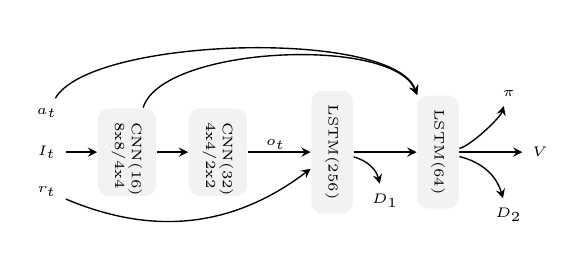
\begin{tikzpicture}
%\draw [use as bounding box] (0,0) rectangle (1.8in, 3in);
\node[networknode] at (7.5, 2.5) (lstm2) {\rotatebox{-90}{LSTM(64)}};
\node[networknode, left=0.8 of lstm2] (lstm) {\rotatebox{-90}{LSTM(256)}};
\node[networknode, left=0.8 of lstm]  (enc2) {\rotatebox{-90}
{\parbox{0.3in}{CNN(32)\\4x4/2x2}}};
\node[networknode, left=0.4 of enc2]  (enc) {\rotatebox{-90}
{\parbox{0.3in}{CNN(16)\\8x8/4x4}}};
\node[left=0.4 of enc] (It) {$I_t$};
\node[above=0.1 of It] (at) {$\actt$};
\node[below=0.1 of It]  (rt) {$\rewt$};
\node [right=0.8 of lstm2] (V)  {$V$};
\node [shift={(-0.4,0)},above=0.4 of V] (pi)  {$\pi$};
\node [shift={(-0.4,0)},below=0.4 of V] (D)  {$D_2$};
\draw [-stealth] (It) edge (enc);
\draw [-stealth] (at) edge [out=60,in=110,looseness=0.5] (lstm2);
\draw [-stealth] (enc) edge [bend left=70,looseness=0.6] (lstm2);
\draw [-stealth] (enc) edge (enc2);
\draw [-stealth] (enc2) edge node [shift={(0.2,0.1)},left]{$o_t$} (lstm);
\draw [-stealth] (rt) edge  [bend right] (lstm);
\draw [-stealth] (lstm) edge node[below=0.4] (D1) {$D_1$} (lstm2);
\draw [-stealth] (lstm) edge [bend left] (D1);
\draw [-stealth] (lstm2) edge [bend right, looseness=0.5] (pi);
\draw [-stealth] (lstm2) edge  (V);
\draw [-stealth] (lstm2) edge [bend left] (D);
\end{tikzpicture}
}%
\end{center}
%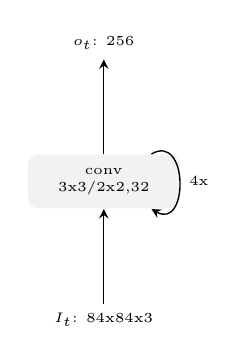
\begin{tikzpicture}
%\draw [use as bounding box] (0,0) rectangle (1.8in, 3in);
\node[] at (2.3, 2) (It) {$I_t$: 84x84x3};
\node[networknode, above=1.2 of It, text width=45, align=center] (c1) {conv\\
  3x3/2x2,32};
\node[above=1.2 of c1] (ft) {$o_t$: 256};
\draw [-stealth] (c1) edge [out=30, in=-30,looseness=2] node [right] {4x}(c1);
\draw [-stealth] (It) -- (c1);
\draw [-stealth] (c1) -- (ft);
\end{tikzpicture}
\hspace{-1ex}%
%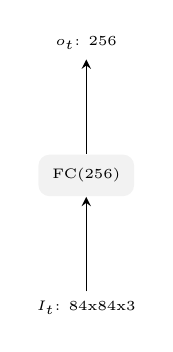
\begin{tikzpicture}
%\draw [use as bounding box] (0,0) rectangle (1.8in, 3in);
\node[] at (2.3, 2) (It) {$I_t$: 84x84x3};
\node[networknode, above=1.2 of It] (fc) {FC(256)};
\node[above=1.2 of fc] (ft) {$o_t$: 256};
\draw [-stealth] (It) -- (fc);
\draw [-stealth] (fc) -- (ft);
\end{tikzpicture}
%
\caption{Modified \NavAiiiCDiDiiL{} (\cite{MiPaViICLR2017}) architecture.
The architecture is has three inputs the current image $I_t$ and previous action $\acttp$ and previous reward $\rewtp$.
As shown by \cite{MiPaViICLR2017}, the architecture improves upon vanilla A3C architecture by using auxiliary outputs of loop-closure signal $L$ and predicted depth $D_1$ and $D_2$.
Since we use a smaller action space than \cite{MiPaViICLR2017} and our agent moves with constant velocity, we do not use velocity at previous time step as input signal.}
\label{fig:architectures}
\end{figure}


\paragraph{Asynchronous Advantage Actor-Critic}
\def\charelig{\nabla_{\theta_\pi}\ln \pit(\acttn; \theta_\pi)}
% There are many different variations of RL. There are many different RL algorithms: value-based methods like Q-learning and SARSA and policy-based method like actor-critic.
In this work, we use the policy-based method called Asynchronous Advantage Actor-Critic (A3C) (\cite{MnBaMiICML2016}), which allows weight updates to happen asynchronously in a multi-threaded environment.
It works by keeping a ``shared and slowly changing copy of target network'' that is updated every few iterations by accumulated gradients in each of the threads.
The gradients are never applied to the local copy of the weights; instead, a local copy of weights is periodically synced from the shared copy of target weights.
The gradient for the weight update is proportional to the product of \emph{advantage}, $R_t - \Value_t(\theta_\Value)$, and \emph{characteristic eligibility}, $\charelig$ (\cite{WiML1992}), which update the weights as
\begin{align}
  \theta_\pi &\leftarrow \theta_\pi
  + \sum_{t \in \text{episode}}\alpha_\pi \nabla_{\theta_\pi}\ln \pit (R_t - \Value_t(\theta_\Value))
  \\
  \theta_\Value &\leftarrow \theta_\Value
  + \sum_{t \in \text{episode}} \alpha_\Value \frac{\partial (R_t - \Value_t(\theta_\Value))^2}
                  {\partial\theta_\Value}
                  \, .
\end{align}

For additional details of the A3C algorithm, we refer the reader to \cite{MnBaMiICML2016}.
\begin{wrapfigure}[20]{r}{0.5\textwidth}
\centering%
\usetikzlibrary{positioning}
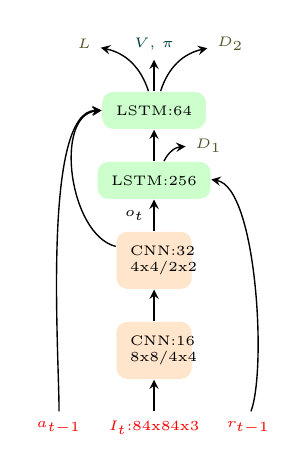
\begin{tikzpicture}
\node[networknode,fill=green!20] at (1.5, 3.5) (lstm2) {LSTM:64};
\node[networknode,fill=green!20,below=0.4 of lstm2] (lstm) {LSTM:256};
\node[networknode,fill=orange!20,below=0.4 of lstm]  (enc2) {\parbox{08ex}{CNN:32\\4x4/2x2}};
\node[networknode,fill=orange!20,below=0.4 of enc2]  (enc) {\parbox{08ex}{CNN:16\\8x8/4x4}};
\node[below=0.4 of enc, inputvar] (It) {$I_t$:84x84x3};
\node[left=0.1 of It,inputvar] (at) {$\acttp$};
\node[right=0.1 of It,inputvar]  (rt) {$\rewtp$};
\node [above=0.4 of lstm2,outvar] (V)  {$V$, $\pi$};
\node [shift={(-0,0)},left=0.3 of V,auxvar] (pi)  {$L$};
\node [shift={(-0,0)},right=0.3 of V,auxvar] (D)  {$D_2$};
\draw [-stealth] (It) edge (enc);
\draw [-stealth] (at) edge [in=-180,out=90,looseness=0.5] (lstm2);
\draw [-stealth] (enc2) edge [bend left=70,in=90,looseness=0.9] (lstm2);
\draw [-stealth] (enc) edge (enc2);
\draw [-stealth] (enc2) edge node [shift={(0,0.0)},left]{$o_t$} (lstm);
\draw [-stealth] (rt) edge  [bend right,in=-110,looseness=0.5] (lstm);
\draw [-stealth] (lstm) edge node[right=0.4,auxvar] (D1) {$D_1$} (lstm2);
\draw [-stealth] (lstm) edge [bend left] (D1);
\draw [-stealth] (lstm2) edge [bend right] (pi);
\draw [-stealth] (lstm2) edge  (V);
\draw [-stealth] (lstm2) edge [bend left] (D);
%\draw [use as bounding box] (0,-1.0) rectangle (3.0, 5.0);
\end{tikzpicture}
%
\caption{Modified \NavAiiiCDiDiiL{} (\cite{MiPaViICLR2017}) architecture.
The architecture is has three inputs the current image $I_t$ and previous action $\acttp$ and previous reward $\rewtp$.
As shown by \cite{MiPaViICLR2017}, the architecture improves upon vanilla A3C architecture by using auxiliary outputs of loop-closure signal $L$ and predicted depth $D_1$ and $D_2$.
Since we use a smaller action space than \cite{MiPaViICLR2017} and our agent moves with constant velocity, we do not use velocity at previous time step as input signal.}
\label{fig:architectures}
\end{wrapfigure}

\paragraph{\NavAiiiCDiDiiL{}}
In this work, we use the \NavAiiiCDiDiiL{} architecture as proposed by \cite{MiPaViICLR2017}, which builds modifying the network architecture to have two LSTMs and with auxiliary outputs of depth predictions along with loop-closure predictions. % TODO "which builds modifying the network architecture..." this doesn't make sense to me, should be corrected.
The schematic of the architecture is shown in Fig~\ref{fig:architectures}.
The architecture has three inputs: the current image $I_t$, previous action $\acttp$ and previous reward $\rewtp$.
As shown by \cite{MiPaViICLR2017}, the architecture improves upon vanilla A3C architecture by optimizing predictions for the auxiliary outputs of loop closure signal $L$ and predicted depth $D_1$ and $D_2$.
Since we use a smaller action space than \cite{MiPaViICLR2017} and our agent moves with constant velocity, we do not use velocity at the previous time step as an input signal.



%\section{Approach}
%% 0. Describe baseline models
% 1. Introduce blinding in a curriculum and finetuning manner
% 2. Introduce the concept of doubling the action space
% 3. Introduce the potential applicablity of this blinding to querying
% the surrounding states of the agent.


\section{Experiments}
% 0. Baseline models
% 1. Blinding is easy enough to understand
% 2. The doubling of the action space - that's the brilliance
%

\begin{table}[h]
    \label{sample-table}
    \begin{center}
        \resizebox{\textwidth}{!}{%
        \begin{tabular}{llllllll}
          \toprule
            Static Goal Mazes & Agent & Reward & Latency 1:$>1$ & Goals & \% Blindfolding & Cont. Blind Frames \\
          \midrule
            \textbf{Static 1} &A3C & 41.01 & 152.3 & 3.48 \\
                              &A3C-CB & 41.01 & 152.3 & 3.48 \\
                              &A3C-FT & 41.01 & 152.3 & 3.48 \\
                              &A3C-BLINC & 41.01 & 152.3 & 3.48 \\
          \midrule
            \textbf{Static 2} &A3C & 41.01 & 152.3 & 3.48 \\
                              &A3C-CB & 41.01 & 152.3 & 3.48 \\
                              &A3C-FT & 41.01 & 152.3 & 3.48 \\
                              &A3C-BLINC & 41.01 & 152.3 & 3.48 \\
          
            \midrule
            \textbf{Static-9x9} &A3C & 41.01 & 152.3 & 3.48 \\
                              &A3C-CB & 41.01 & 152.3 & 3.48 \\
                              &A3C-FT & 41.01 & 152.3 & 3.48 \\
                              &A3C-BLINC & 41.01 & 152.3 & 3.48 \\
          \bottomrule
        \end{tabular}}
    \end{center}
    \caption{We achieve comparable results when we test and train on the same experiments.}
\end{table}

\begin{table}[h]
    \label{sample-table}
    \begin{center}
        \resizebox{\textwidth}{!}{%
        \begin{tabular}{llllllll}
          \toprule
            Random Goal Mazes & Agent & Reward & Latency 1:$>1$ & Goals & \% Blindfolding & Cont. Blind Frames \\
          \midrule
            \textbf{Random 1} & 41.01 & 152.3 & 3.48 \\
                              & 41.01 & 152.3 & 3.48 \\
                              & 41.01 & 152.3 & 3.48 \\
                              & 41.01 & 152.3 & 3.48 \\
          \midrule
            \textbf{Random 2} & 41.01 & 152.3 & 3.48 \\
                              & 41.01 & 152.3 & 3.48 \\
                              & 41.01 & 152.3 & 3.48 \\
                              & 41.01 & 152.3 & 3.48 \\
          \midrule
            \textbf{Random-9x9-10} & 41.01 & 152.3 & 3.48 \\
                              & 41.01 & 152.3 & 3.48 \\
                              & 41.01 & 152.3 & 3.48 \\
                              & 41.01 & 152.3 & 3.48 \\
          \bottomrule
        \end{tabular}}
    \end{center}
    \caption{We achieve comparable results when we test and train on the same experiments.}
\end{table}


\subsection{Blinding: Curriculum and Finetuning}

\subsection{Blinding: Self-Supervised Curriculum Training}



\section{Analysis}
\begin{figure}%
  \includegraphics[width=\linewidth]{images/plot_summary_bar_plots.pdf}%
  \caption{
    We evaluate the \NavAiiiCDiDiiL{}~\cite{MiPaViICLR2017} algorithm on ten randomly chosen maps, shown in Fig.~\ref{fig:evironments}, with increasing difficulty as described in Sec.~\ref{sec:navtasks}.
    The figure is best viewed in color.
    Vertical axis is one of the ten map ID's on which the agent was trained (except for Rnd. Maze) and evaluated.
    Horizontal axis are different evaluation metrics.
    We note that when the goal is static then rewards are consistently higher as compared to random goal.
    With static goals, the metric \DistanceInefficiency{} is close to 1,
    indicating that the algorithms are able to find shortest path.
    However, with random goals, the agents struggle to find the shortest path.
    From the \LatencyOneGtOne{} results we note that the algorithm do well when trained and tested on the same map but fail to generalize to new maps when evaluated on ability to exploit the information about goal location.
    Also note that \LatencyOneGtOne{} metric for cases of static goals is expected to be close to one because the location of goal is learned at train time.
  }%
\label{fig:latency-goal-reward}%
\end{figure}

\begin{figure}[t!]%
\centering%
\def\figw{0.16\columnwidth}%
\newcommand{\includesnapshot}[1]{%
  \includegraphics[width=\figw,trim=336pt 0 0 0,clip]{#1}}%
\includesnapshot{images/snapshot/00063000-snapshot.png}%
\includesnapshot{images/snapshot/00087000-snapshot.png}%
\includesnapshot{images/snapshot/00156165-snapshot.png}%
\includesnapshot{images/snapshot/00159840-snapshot.png}%
\includesnapshot{images/snapshot/00166605-snapshot.png}%
\includegraphics[width=\figw]{images/dhiman_0002_entityLayer.pdf}\\
\includesnapshot{images/snapshot/00193065-snapshot.png}%
\includesnapshot{images/snapshot/00338220-snapshot.png}%
\includesnapshot{images/snapshot/00344985-snapshot.png}%
\includesnapshot{images/snapshot/00948930-snapshot.png}%
\includesnapshot{images/snapshot/00956325-snapshot.png}%
\includegraphics[width=\figw]{images/dhiman_0003_entityLayer.pdf}\\

\caption{The ten randomly chosen mazes for evaluation. We generate 1100 random mazes and choose ten to evaluate our experiments that require testing and training on the same maps.}%
\label{fig:environments}
\end{figure}

\subsection{Metric Evaluations}
\paragraph{Static goal, static spawn, static maze} In this simplest case, the agents memorizes the a path to the goal during training and repeats it during testing. The reward is high, and both the \LatencyOneGtOne{} and distance-efficiency is close to 1 with small standard deviations implying the path chosen is the shortest available.

\paragraph{Static goal, random spawn, static map} The agent must memorize the goal's location and learn to traverse to it from different parts of the map. The large deviations in the \LatencyOneGtOne{} indicate that the agent is able to better traverse to the goal from certain sections of the map implying that the goal-exploitation ability is not uniform to every spawn location. The distance-efficiency is close to 1 implying that when the goal is found, the shortest path is traversed.

\paragraph{Random goal, static spawn, static map} The goal is randomized and must be found at evaluation time. The mean of the \LatencyOneGtOne{} is more than 1 show that in general the agent is able to exploit map information. However the large standrd deviations in this metric and the reward values show that this exploitation is not consistent through episodes. For most of the experiments, the distance-efficiency is close to one within error metrics, again imply that the shortest path is taken when the goal is found. 

\paragraph{Random goal, Random spawn, static map} Similar to the previous experiment, the \LatencyOneGtOne{} is more than 1 but with a large standard deviation implying inconsistent performance from episode to episode. The distance efficiency is larger than 1 showcasing the paths traversed to the goal are not necessarily the shortest.

\paragraph{Random goal, Random spawn, Random map} Agents trained on a 1000 maps are tested individually on the 10 chosen maps. The \LatencyOneGtOne{} is close to 1 implying that map-exploitation is taking place. The large distance-efficiency numbers seem to confirm this statement. Qualitatively, based on video results, the agents appear to randomly explore the maze in the direction of initiialization.


\subsection{Evaluation on unseen maps}
The results for training on $N$ maps, where $N \in \{10, 100, 500, 1000\}$, and testing on 100 unseen maps are shown in Fig~\ref{fig:num-training-maps}.
We observe that there is a significant jump of average reward and average goal hits when the number of training maps is increased from 10 to 100 but no significant increase when the number of training maps are increased from 100 to 500 to 1000.
This is due to the fact that the wall-following strategy learned by the algorithm,
is learned with enough variation in 100 maps and training on additional maps does not add to the learned strategy.

\subsection{Effect of apples and texture}
We evaluate the effect of apples and texture during evaluation time in Fig~\ref{fig:num-training-maps}.
We train the algorithm on randomly chosen training maps with random texture and evaluate them no maps with and without random texture and also on maps with and without apples. When the apples are present, we place the apples with probability 0.25 in each block of the map.
We find that the algorithm, being trained on random textures and random placement of apples, is robust to presence or absence of textures and apples.


\subsection{Qualitative evaluation on simple maps}
% 1. We test the trained algorithms on simple maps.
To evaluate what strategies that the algorithm is employing to reach the
goal we evaluate the algorithm on very simple maps where there are only two
paths to reach the goal. The qualitative results for the evaluation are shown
in Fig~\ref{fig:planning-qualitative}.

\begin{figure}%
  \includegraphics[width=\linewidth]{images/plot_ntrain_summary.pdf}%
  \caption{Plots showing the effect of number of training maps with random texture (Rnd Texture) and presence of apples (With apples), when evaluated on unseen maps. We note that although the difference between mean metrics is negligible as compared to standard deviation of the metrics. Hence we say that the effect of apples or textures can be ignored.
  The only clear trend is apparent \LatencyOneGtOne{} metric which suggest that random texture along without apples is advantageous in exploiting goal location while finding the goal second time on-wards.}
  \label{fig:num-training-maps}
\end{figure}

\paragraph{Square map}
% 3. In the square map, we find that the path taken is in the
%    direction of pose initialization. the visualization of path taken is
%    shown in Fig. . the correlation with of path taken with initial pose
%    is shown in Fig. . The correlation with shortest path is shown in
%    Fig. . Hence, the algorithm instead of shortest path planning takes the
%    the direction in which it is initialized.
A Square map (Fig~\ref{fig:planning-qualitative}) is the simplest possible map with two paths to the goal.
We evaluate the algorithm trained on 1000 random maps on square map.
We observe that the agent greedily moves in the direction of
initialization.
This may be because of the initial learning which is
motivated by small rewards of getting apples.
We compute the percentage of times the agent takes the shortest path over a trial of 100 episodes.
We find the agent takes the shortest path only $50.4$\% ($\pm 12.8$\%) of the times, no better than random.
% Quantitative result taken from:
% exp-results/planning-09x09-0002/gen_stats_latest_loaded-from-training-1000_acting-on-planning-09x09-0002_vars-True_apples-0.json

\paragraph{Wrench map}
% 2.2 To eliminate the correlation with initial orientation, we start
%     with wrench map. The spawn point is guaranteed to be initialized in
%     the handle of the wrench. Hence, the decision point is the only
%     junction in the map where the algorithm either decides to take a
%     left or a right.
%     We find no correlation between shortest path and the direction taken. 
To eliminate the dependency on initial orientation, we evaluate the algorithm on Wrench map as shown in Fig~\ref{fig:planning-qualitative}. We fix in the spawn point at the bottom of the tail so that shortest path is independent of the spawn orientation.
The decision about the shortest path is made at the junction where the agent can either chose to go left or right.
We find that the agent is taking shortest path only $32.9$\% ($\pm 25.1$\%) of the times which is again to better than random.
% Quantitative result taken from:
% exp-results/planning-09x09-0004/gen_stats_latest_loaded-from-training-1000_acting-on-planning-09x09-0004_vars-True_apples-0.json

% Goal map provides a similar independence from starting orientation
% but the penalty for choosing the wrong path is much higher than the
% wrench map. 
\paragraph{Goal map}
Similarly to the wrench map, the goal map (Fig~\ref{fig:planning-qualitative}) provides a decision point independent of the initial orientation, but it penalizes the wrong decision more than the wrench map $42.6$\% ($\pm 35.1$\%) of the times which is again no better than random.
% Quantitative result taken from:
% exp-results/planning-09x09-0006/gen_stats_latest_loaded-from-training-1000_acting-on-planning-09x09-0006_vars-True_apples-0.json

% JJC: TODO: Summarize results on simple maps
These experiments show that \NavAiiiCDiDiiL{} algorithm, even when trained on 1000 maps, do not generalize to these very simple maps.
Again note that even in cases when there are only two possible paths to the goal, the agent is unable to chose the shorter path with more than 50\% probability.
This shows that the models trained on 1000 maps have learned only a wall-following strategy rather than learning to plan path based on goal location.

%\subsubsection{Qualitative results}
\begin{figure}[h]
\def\vertspace{1em}
\rotatebox{90}{\hspace{3em}Square map}%
\includegraphics[width=0.98\textwidth]{./exp-results/training-1000_on_square_map.png}%
\vspace{\vertspace}
\rotatebox{90}{\hspace{4em}Wrench map}%
\includegraphics[width=0.98\textwidth]{./exp-results/training-1000_on_wrench_map.png}%
\vspace{\vertspace}
\rotatebox{90}{\hspace{5em}Goal map}%
\includegraphics[width=0.98\textwidth]{./exp-results/training-1000_on_goal_map.png}%
\caption{Qualitative results when model trained on 1000 maps is
  evaluated on unseen simple maps.
  In this particular example, the agent takes the shortest path 6/10 times but when averaged over 100 episodes, the percentage of shortest path taken is reduced to $50.4$\% ($\pm 12.8$\%).
  Although for the example of wrench map the agent takes the shortest path 8/10 times but when averaged over 100 episodes, the percentage of shortest path taken is reduced to $32.9$\% ($\pm 25.1$\%).
 For the goal map, the example chosen here shows that the shortest path is only taken 1/6 times, on an average over 100 episodes, the shortest path is taken $42.6$\% ($\pm 35.1$\%) times.
}
\label{fig:planning-qualitative}
\end{figure}


\subsection{Attention Maps}
We use the normalized sum of absolute gradient of the loss with respect to the input image as a proxy for attention in the image.
The gradients are normalized for each image so that the maximum gradient is one. The attention values are then used as a soft mask on the image to create the visualization as shown in Fig~\ref{fig:attention}

We observe that the attention is uniformly distributed on the image when the agent spawns. The attention narrows down to a few pixels in the center when the agent is navigating through the corridor. It spreads to the entire image around turns and junctions. The attention also pays close attention to important objects like goal, apples and unique decals.

\begin{figure}
\includegraphics[width=\textwidth,trim=0 0 0 336pt,clip]{./exp-results/training-09x09-0127-on-0127.png}\vspace{1ex}\\
%
\includegraphics[width=\textwidth,trim=0 0 0 336pt,clip]{./exp-results/training-1000-on-0127.png}%
\caption{Visualizing attention for two sequences. The first two rows show the sequin when the model is trained on and evaluated on the same map. The last two rows shows the sequence for a model trained on 1000 maps and evaluated on one of the maps. We observe that the attention is uniformly distributed on the image when the agent spawns. The attention narrows down few pixels in the center when the agent is navigating through the corridor. It spreads to the entire image around turns and junctions. The attention also pays close attention to important objects like goal, apples and unique decals.}
\label{fig:attention}
\end{figure}


%Are we close to replacing the classic mapping and path-planning algorithms with DRL algorithms?
%
%As shown by the results in Fig~\ref{fig:latency-goal-reward}, the state of art DRL algorithm works well if trained and tested on the same map (static map), but performance reaches to the level of simple bug exploration like algorithms if training and testing are on different maps.





\section{Conclusion}
In this work we show that state of art Deep reinforcement learning algorithms do not peroform long term mapping and or path planning.
We provide evidence that the algorithms are learning to perform bug exploration algorithm when the position of goal is random. When the position of goal and structure of map is known at training time, then the Deep reinforcement learning algorithms
are able to learn near optimal policy and able to repeat it at test time.


\begin{figure}%
  \includegraphics[width=\linewidth]{images/plot_ntrain_summary.pdf}%
  \vspace{-1em}%
  \caption{Plots showing the effect of number of training maps with random texture (Rnd Texture) and presence of apples (With apples), when evaluated on unseen maps. We note that although the difference between mean metrics is negligible as compared to standard deviation of the metrics. Hence we say that the effect of apples or textures can be ignored.
  The only clear trend is apparrent \LatencyOneGtOne{} metric which suggest that random texture along without apples is advantageous in exploiting goal location while finding the goal second time onwards.}
  \label{fig:num-training-maps}
\end{figure}

\subsubsection*{Acknowledgments}

Use unnumbered third level headings for the acknowledgments. All
acknowledgments, including those to funding agencies, go at the end of the paper.

{\small
\IfFileExists{/z/home/dhiman/wrk/group-bib/shared.bib}{
  \bibliography{/z/home/dhiman/wrk/group-bib/shared,main,main_filtered}
}{
  \bibliography{main,main_filtered}
}
\bibliographystyle{iclr2018_conference}
}

\newpage
\subsubsection{Qualitative results}
\begin{figure}[h]
\rotatebox{90}{\hspace{3em}Square map}%
\includegraphics[width=0.98\textwidth]{./exp-results/training-1000_on_square_map.png}%
\vspace{1pt} \hrule \vspace{1pt}%
\rotatebox{90}{\hspace{4em}Wrench map}%
\includegraphics[width=0.98\textwidth]{./exp-results/training-1000_on_wrench_map.png}%
\vspace{1pt} \hrule \vspace{1pt}%
\rotatebox{90}{\hspace{5em}Goal map}%
\includegraphics[width=0.98\textwidth]{./exp-results/training-1000_on_goal_map.png}%
\caption{Qualitative results when model trained on 1000 maps is
  evaluated on unseen simple maps.
  In this particular example, the agent takes the shortest path 6/10 times but when averaged over 100 episodes, the percentage of shortest path taken is reduced to $50.4$\% ($\pm 12.8$\%).
  Although for the example of wrench map the agent takes the shortest path 8/10 times but when averaged over 100 episodes, the percentage of shortest path taken is reduced to $32.9$\% ($\pm 25.1$\%).
 For the goal map, the example chosen here shows that the shortest path is only taken 1/6 times, on an average over 100 episodes, the shortest path is taken $42.6$\% ($\pm 35.1$\%) times.
}
\label{fig:planning-qualitative}
\end{figure}
\end{document}
